\documentclass[12pt]{article}
\usepackage{amsmath}
\usepackage{amssymb}
\usepackage{enumerate}
\usepackage{geometry}
\usepackage{tikz}
\usetikzlibrary{automata, positioning, arrows}
\geometry{margin=1in}

\title{Problem Set 4 - CPSC 326\\Solutions}
\author{Fernando, Dang, Raj, Eric M.}
\date{\today}

\begin{document}
\maketitle

\section*{Problem 1}
Consider the following Language:
$$L_1 = \{w \in \{a, b, c, d\}^* \mid (w \text{ contains the strings } abb \text{ and } bbc) \text{ or } (w \text{ contains the string } abc)\}$$

Develop a NFA for $L_1$.

\textbf{Answer:}

The NFA uses nondeterminism to check for either:
\begin{itemize}
    \item Case 1: Both $abb$ and $bbc$ appear in $w$
    \item Case 2: $abc$ appears in $w$
\end{itemize}

\textbf{States:}
\begin{itemize}
    \item $q_0$: Initial state
    \item $q_1, q_2, q_3$: Track progress toward finding $abb$
    \item $q_4, q_5, q_6$: Track progress toward finding $bbc$ (after finding $abb$)
    \item $q_7$: Found both $abb$ and $bbc$ (accepting)
    \item $q_8, q_9, q_{10}$: Track progress toward finding $abc$
    \item $q_{11}$: Found $abc$ (accepting)
\end{itemize}

\textbf{NFA Diagram:}

\begin{center}
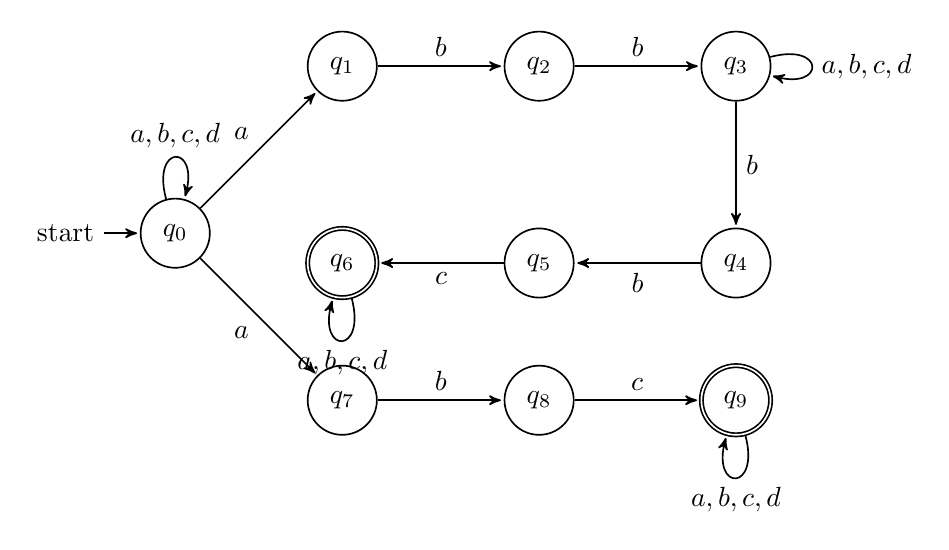
\begin{tikzpicture}[>=stealth', shorten >=1pt, auto, node distance=2.5cm, semithick]
    % Initial state
    \node[state, initial] (q0) {$q_0$};
    
    % Path for abb
    \node[state] (q1) [above right of=q0, node distance=3cm] {$q_1$};
    \node[state] (q2) [right of=q1] {$q_2$};
    \node[state] (q3) [right of=q2] {$q_3$};
    
    % Path for bbc (after abb)
    \node[state] (q4) [below of=q3] {$q_4$};
    \node[state] (q5) [left of=q4] {$q_5$};
    \node[state, accepting] (q6) [left of=q5] {$q_6$};
    
    % Path for abc
    \node[state] (q7) [below right of=q0, node distance=3cm] {$q_7$};
    \node[state] (q8) [right of=q7] {$q_8$};
    \node[state, accepting] (q9) [right of=q8] {$q_9$};
    
    \path[->]
    % Self-loop on start
    (q0) edge [loop above] node {$a,b,c,d$} (q0)
    
    % Path to find abb
    (q0) edge node [above left] {$a$} (q1)
    (q1) edge node {$b$} (q2)
    (q2) edge node {$b$} (q3)
    (q3) edge [loop right] node {$a,b,c,d$} (q3)
    
    % From q3, find bbc
    (q3) edge node [right] {$b$} (q4)
    (q4) edge node {$b$} (q5)
    (q5) edge node {$c$} (q6)
    (q6) edge [loop below] node {$a,b,c,d$} (q6)
    
    % Path to find abc directly
    (q0) edge node [below left] {$a$} (q7)
    (q7) edge node {$b$} (q8)
    (q8) edge node {$c$} (q9)
    (q9) edge [loop below] node {$a,b,c,d$} (q9);
\end{tikzpicture}
\end{center}

\textbf{Explanation:}
The NFA nondeterministically chooses between:
\begin{itemize}
    \item Following the upper path to find $abb$, then continuing to find $bbc$
    \item Following the lower path to find $abc$
\end{itemize}
Once either accepting state is reached, the string is accepted.

\newpage

\section*{Problem 2}
Let $L_2 = \{w \in \{a, b, c\}^* \mid w = (abc)^*a^*\}$. Design a NFA that accepts the language $L_2$.

\textbf{Answer:}

The language consists of zero or more repetitions of $abc$, followed by zero or more $a$'s.

\textbf{States:}
\begin{itemize}
    \item $q_0$: Initial and accepting state
    \item $q_1$: Just read $a$ (could be start of $abc$ or final $a$'s)
    \item $q_2$: Read $ab$ (continuing $abc$)
    \item $q_3$: Read $abc$ (back to accepting, or continue with more $a$'s)
\end{itemize}

\textbf{NFA Diagram:}

\begin{center}
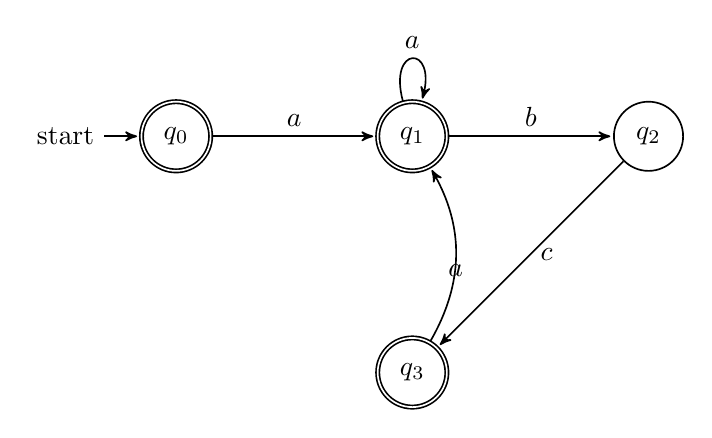
\begin{tikzpicture}[>=stealth', shorten >=1pt, auto, node distance=3cm, semithick]
    \node[state, initial, accepting] (q0) {$q_0$};
    \node[state, accepting] (q1) [right of=q0] {$q_1$};
    \node[state] (q2) [right of=q1] {$q_2$};
    \node[state, accepting] (q3) [below of=q1] {$q_3$};
    
    \path[->]
    (q0) edge node [above] {$a$} (q1)
    (q1) edge node [above] {$b$} (q2)
    (q2) edge node [right] {$c$} (q3)
    (q3) edge [bend right=30] node [below] {$a$} (q1)
    (q1) edge [loop above] node {$a$} (q1);
\end{tikzpicture}
\end{center}

\textbf{Explanation:}
\begin{itemize}
    \item From $q_0$, we can either accept immediately ($\varepsilon$ is in the language) or read $a$
    \item After reading $a$, we nondeterministically choose:
    \begin{itemize}
        \item Continue with $bc$ to complete an $abc$ block
        \item Stay in $q_1$ reading more $a$'s (the final $a^*$ part)
    \end{itemize}
    \item After completing $abc$ (reaching $q_3$), we can start another $abc$ block or accept
    \item States $q_0$, $q_1$, and $q_3$ are accepting to handle $(abc)^*a^*$ properly
\end{itemize}

\newpage

\section*{Problem 3}
Let $L_3 = \{w \in \{0, 1, 2, 3, 4, 5, 6, 7, 8, 9\}^* \mid \text{the final digit of the string } w \text{ has not appeared before in } w\}$.

Design a NFA that accepts the language $L_3$.

\textbf{Answer:}

The NFA uses nondeterminism to guess which digit will be the final digit that hasn't appeared before.

\textbf{Strategy:}
The NFA nondeterministically guesses which digit will appear for the first time at the end. For each possible final digit, we have a separate branch that:
\begin{itemize}
    \item Reads any other digits (but not that specific digit)
    \item Reads that specific digit once at the end
    \item Accepts
\end{itemize}

\textbf{States:}
\begin{itemize}
    \item $q_{\text{start}}$: Initial state
    \item For digit 0: $q_{0a}$ (reading, avoiding 0), $q_{0b}$ (just read 0, accepting)
    \item For digit 1: $q_{1a}$ (reading, avoiding 1), $q_{1b}$ (just read 1, accepting)
    \item For digit 2: $q_{2a}$ (reading, avoiding 2), $q_{2b}$ (just read 2, accepting)
    \item $\ldots$ (similar for digits 3-9)
    \item For digit 9: $q_{9a}$ (reading, avoiding 9), $q_{9b}$ (just read 9, accepting)
\end{itemize}

\textbf{NFA Diagram:}

\begin{center}
    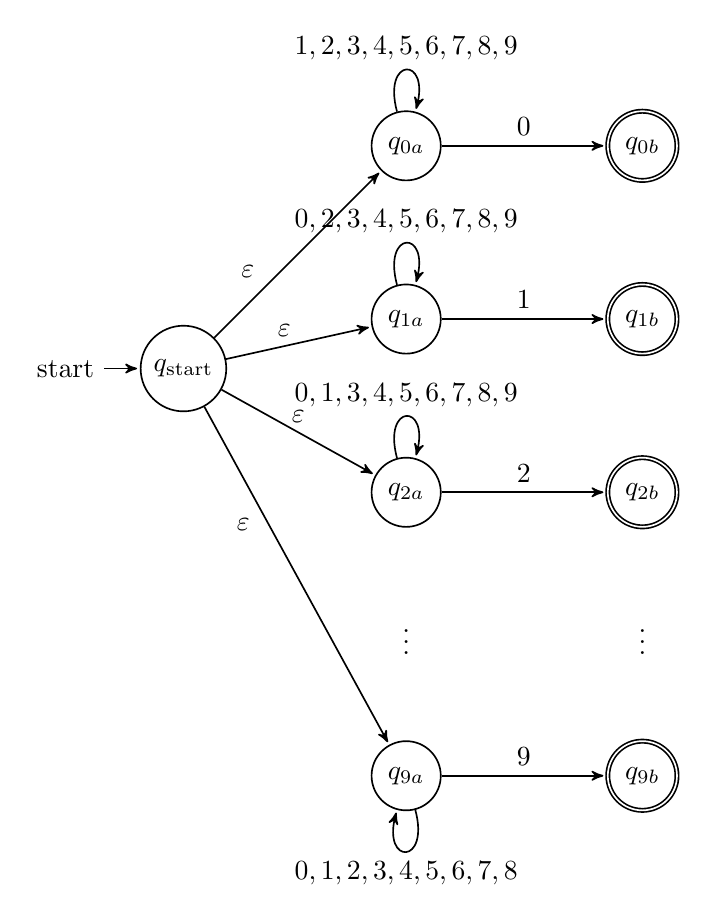
\begin{tikzpicture}[>=stealth', shorten >=1pt, auto, node distance=4cm, semithick]
        \node[state, initial] (start) {$q_{\text{start}}$};
        
        % Branch for digit 0
        \node[state] (q0a) [above right of=start, node distance=4cm] {$q_{0a}$};
        \node[state, accepting] (q0b) [right of=q0a, node distance=3cm] {$q_{0b}$};
        
        % Branch for digit 1
        \node[state] (q1a) [below of=q0a, node distance=2.2cm] {$q_{1a}$};
        \node[state, accepting] (q1b) [right of=q1a, node distance=3cm] {$q_{1b}$};
        
        % Branch for digit 2
        \node[state] (q2a) [below of=q1a, node distance=2.2cm] {$q_{2a}$};
        \node[state, accepting] (q2b) [right of=q2a, node distance=3cm] {$q_{2b}$};
        
        % Dots to indicate more branches
        \node (dots1) [below of=q2a, node distance=1.8cm] {$\vdots$};
        \node (dots2) [below of=q2b, node distance=1.8cm] {$\vdots$};
        
        % Branch for digit 9
        \node[state] (q9a) [below of=dots1, node distance=1.8cm] {$q_{9a}$};
        \node[state, accepting] (q9b) [right of=q9a, node distance=3cm] {$q_{9b}$};
        
        \path[->]
        % Epsilon transitions from start to each branch
        (start) edge node [above left, pos=0.3] {$\varepsilon$} (q0a)
        (start) edge node [above, pos=0.4] {$\varepsilon$} (q1a)
        (start) edge node [above, pos=0.5] {$\varepsilon$} (q2a)
        (start) edge node [below left, pos=0.3] {$\varepsilon$} (q9a)
        
        % Branch 0: read anything except 0, then read 0
        (q0a) edge [loop above] node {$1,2,3,4,5,6,7,8,9$} (q0a)
        (q0a) edge node [above] {$0$} (q0b)
        
        % Branch 1: read anything except 1, then read 1
        (q1a) edge [loop above] node {$0,2,3,4,5,6,7,8,9$} (q1a)
        (q1a) edge node [above] {$1$} (q1b)
        
        % Branch 2: read anything except 2, then read 2
        (q2a) edge [loop above] node {$0,1,3,4,5,6,7,8,9$} (q2a)
        (q2a) edge node [above] {$2$} (q2b)
        
        % Branch 9: read anything except 9, then read 9
        (q9a) edge [loop below] node {$0,1,2,3,4,5,6,7,8$} (q9a)
        (q9a) edge node [above] {$9$} (q9b);
    \end{tikzpicture}
    \end{center}

\textbf{Explanation:}

The NFA has 21 total states: 1 start state + 10 branches (one for each digit 0-9), where each branch has 2 states.

How it works:
\begin{enumerate}
    \item From $q_{\text{start}}$, use $\varepsilon$-transitions to nondeterministically guess which digit will be the final new digit
    \item If we guess digit 0 will be the final new digit:
    \begin{itemize}
        \item Go to state $q_{0a}$
        \item Loop in $q_{0a}$ reading any digit 1-9 (but never 0)
        \item Read 0 and go to accepting state $q_{0b}$
    \end{itemize}
    \item If we guess digit 1 will be the final new digit:
    \begin{itemize}
        \item Go to state $q_{1a}$
        \item Loop in $q_{1a}$ reading any digit except 1
        \item Read 1 and go to accepting state $q_{1b}$
    \end{itemize}
    \item Similar logic applies for guessing digits 2 through 9
\end{enumerate}

\textbf{Example:}

For string $w = 237$ (where 7 appears for the first time at the end):
\begin{itemize}
    \item Start: $q_{\text{start}}$
    \item Guess 7 is final: $q_{\text{start}} \xrightarrow{\varepsilon} q_{7a}$
    \item Read 2: $q_{7a} \xrightarrow{2} q_{7a}$
    \item Read 3: $q_{7a} \xrightarrow{3} q_{7a}$
    \item Read 7: $q_{7a} \xrightarrow{7} q_{7b}$ (accept)
\end{itemize}

For string $w = 5$ (single digit, first occurrence):
\begin{itemize}
    \item Start: $q_{\text{start}}$
    \item Guess 5 is final: $q_{\text{start}} \xrightarrow{\varepsilon} q_{5a}$
    \item Read 5: $q_{5a} \xrightarrow{5} q_{5b}$ (accept)
\end{itemize}

\end{document}